
\chapter{INTRODUCTION}
The SOM is a type of artificial neural network developed by \cite{Kohonen2000}. 
Artificial neural networks are a broad class of mathematical or computational
models conceptually based on biological neural networks.  The SOM is based in part
on ideas about the learning process found in biological neural networks.  In
the SOM an input-space is organized onto a set of neurons through an unsupervised
competitive learning process.  Neurons compete for input signals and winning
neurons are updated to better model these signals. As the learning progresses
similar input signals are attracted to similar areas of the network.

The SOM has a number of applications and is primarily used for data reduction
and data visualization.  Other data reductions techniques, such as principle
components or multi-dimensional scaling, reduce the dimensionality of 
the input-space, but do not preform clustering.  The SOM on the other hand has
the ability to do both simultaneously.  The degree to which clustering occurs
is controlled by the size of the SOM.

\cite{skupin08} demonstrate the clustering properties of SOM when they use
state level data from the U.S. Census Bureau to train a three-by-three (9)
neuron SOM.  The neurons act as containers clustering similar states.  In a
similar experiment they train a twenty-by-twenty (400) neuron SOM with same
data.  In this case the SOM proves to be a very useful visualization tool,
providing a low-dimensional spatial layout of otherwise high-dimensional data.

A useful property of the SOM is that the network structure between the neurons
allows us to create meaningfull visualisations.  Observations used in the
training, as wells as new observations from the input space,  can be mapped
onto the trained surface in order to show higher dimension relationships in a
familiar map-like form. The SOM's component planes captures the spacial layout
in each dimmension, these are often visualized in a series of maps.  These
maps can provided useful information about the relationships between the
difference attirubtes of your input-space.

\subsection{SOM Training}
The leaning process in SOM is often described a training.  We must train the
neurons in the network to better represent the input-space.  This is done
through an interative process, where each observation from the input-space is
given several opertunites to affect the SOM's neurons.  Each neuron in the SOM
is said to model a portion of the input-space \cite{Kohonen2000}. To acomplish
this each neuron is associated with a parametric reference vector, \(m_i\)
\cite{Kohonen2000}.  The parameters of these vecotors are adjusted during
training such that they begin the model the inputs assigned to them.




Intro The SOM, 
	THE SOM
		what it is.
			ANN
				what they are. (Need a lit review here).
			Learning Process
		what it's used for, 
			Clustering
				How this works
			Data Reduction
				How this works
			Data Visualization
				How this works
		how it works.
			input data
			training process
		limitations of the som.
			edges
		

The Self-Organizing Map (SOM) is an unsupervised competitive learning process
developed by Teuvo Kohonen.
The technique is generally used on high-dimensional data

to analyze and visualize high dimensional data sets.  
Applications of SOM generally fall under three catagories; data visualization, data reduction and clustering.  



The applications of SOM are far reaching; \cite{Kohonen2000} provides a thorough review of the SOM literature including applications of SOM.  

SOM has been used in applications ranging from speech recognition and image classification to breast cancer detection and gene expression clustering.  

\cite{skupin08} outline the growing interest of SOM to
the GISciences, and propose that the relationship between SOM and GIScience
should be bidirectional.  The SOM offers a powerful method for exploring and
visualizing geographic data and GIScience offers a wide array of tools
and methods to enable the exploration of the SOM itself.  This thesis takes
advantage of GeoVisualization and GeoCompution in order to explore some of the basic
properties of the SOM.

The SOM is a type of artificial neural network in which neurons are ``organized''
in such a way as to project the high-dimensional relationships of a set of
training data onto a low-dimensional network structure.  The traditional
SOM uses a rectangular or hexagonal network topology \citep{Kohonen2000}.  These topologies 
create a well-known problem in SOM called the boundary or edge effect.  Neurons on
the boundary of the hexagonal and rectangular lattices have fewer neighbors,
which reduces their ability to interact with other neurons during the
self-organizing process.  Using a spherical lattice has been widely suggested as a
solution to the problem \citep{ritter99, boudjemai2003, sangole03,
Nishio:2006fk, wu2006}. The use of the spherical lattice, however, does not
completely overcome the boundary problem, and the choice of which spherical
topology to use for the network can be difficult to make.

A regular network topology is one in which every node on the network has exactly the
same number of adjacent nodes.  Any topology involving an edge is irregular.
Arranging our lattice on the surface of a sphere seems to be an obvious
way to overcome the edge.  However, there exist only five arrangements on the
sphere which are completely regular; these are the five platonic solids \citep{ritter99,
harris2000}.  Any other arrangement of neurons on the surface of the sphere will
result in an irregular topology, as not all neurons will have the same number of
neighbors.  The classic method for minimizing this irregularity is to generate
the spherical lattice by tessellating the sides of the icosahedron
\citep{Nishio:2006fk}.  While this method will always result in a highly
regular spherical topology, the main drawback is that the number of neurons in
the network (the network size), \(N\), grows exponentially as tessellations are
applied. That results in only very coarse control over network size.
 Other methods for arranging neurons on the sphere allow
for unlimited control over network size, but yield topologies with increased
irregularity \citep{harris2000, wu2005, Nishio:2006fk}.  To date the
literature has largely ignored the more irregular methods in favor of the
aforementioned tessellation-based methods.  A topology which yields a more flexible network
size may be desirable.  However, in order to address this issue of network
size, we must first determine the degree to which irregularity effects the
SOM.

\section{Research Objectives}
The objective of this research is to determine the utility of certain irregular
spherical topologies beyond offering greater control over network size.  Toward
that end, I develop and test new diagnostics to measure and visualize
topology-induced errors in SOM.  The following diagnostics are developed and
implemented:

\begin{enumerate}
    	\item Compare the internal variance of observations captured by a given neuron to that neuron's first-order neighborhood size.
	\item For different topologies, compare the internal variance of each neuron against a composite measure of topological regularity.
	\item Develop a SOM-based visualization of the internal variance.
	%\item Develop a reverse quantization error visualization by mapping neurons back onto the input data.
\end{enumerate}

These diagnostics help facilitate the evaluation of both traditional and
spherical SOMs.  To satisfy the objective of this research, I apply these
diagnostics to a series of comparable SOMs.  Each SOM is trained using the
same synthetic data and training parameters, but utilize different network
topologies.  By formally testing for difference of means and variance in the
results of the diagnostics, the following questions are addressed:

%topologies.  By formally testing for statistical differences in the
%results of the diagnostics the following questions will be addressed:
\begin{enumerate}
	\item Does the internal variance of a neuron decrease as its first-order neighborhood size, or degree, increases?
	\item Is the average internal variance of a SOM higher when a more irregular topology is used?
	\item Which insights, if any, can be gained from a SOM-based visualization of internal variance?
\end{enumerate}



\chapter{BACKGROUND}
This chapter is divided into four sections.  The first provides a general
introduction to the SOM algorithm and the problems created by using irregular
topology. The second reviews the current spherical topologies used with SOMs.
The third examines the flexibility of the various topologies with regard to
network size. The fourth takes a look at the limitations of using ``uniformity''
to evaluate potential topologies.

\section{Training}
The SOM is a type of artificial neural network, in the SOM high-dimensional
data are organized onto a low-dimensional lattice, or map, of neurons.  The
structure of the lattice is referred to as the topology of the SOM.  This
topology defines how the neurons in the SOM will interact with each other.


 the interaction that takes place within the SOM and will
be described in detail later in this chapter.  

The SOM algorithm uses an artificial neural network to organize
high-dimensional data onto a low-dimensional lattice, or map, of neurons.
Each neuron contains a reference vector that models the input data.  Before
training, these neuron-vectors are initialized, most commonly to random
values.  During the training process a randomly selected observation (input
vector $x$) searches all neurons (reference vectors $m_i$) to find the one to
which it is most similar, referred to as its Best Matching Unit (BMU $c$).
The BMU and its neighborhood ($N_c$) are then adjusted to better match that
observation \citep{Kohonen2000}.  The training process is repeated a
predefined number of times, or ideally until the map converges. The
traditional SOM is laid out on a two-dimensional plane using either a
rectangular or hexagonal topology.  According to \cite{wu2006}, the hexagonal
structure is more uniform and generally preferred.

One drawback of building the neural lattice in a discrete Euclidean plane is the
boundary of the resulting lattice.  A neuron located on the boundary has fewer
neighbors and thus fewer chances of being updated \citep{wu2006}.  As observed
in Figure \ref{figure1}, neurons in the center of the map tend to better
represent the mean of the input-space.  This is arguably caused by outliers
being pushed to the edges of the map, where they encounter fewer competing
signals.
% Skupin's Comment here is not addressed.  Not sure if it needs a response or
% simply an acknowledgement.


\section{The Boundary Effect}


\begin{figure}
\centering
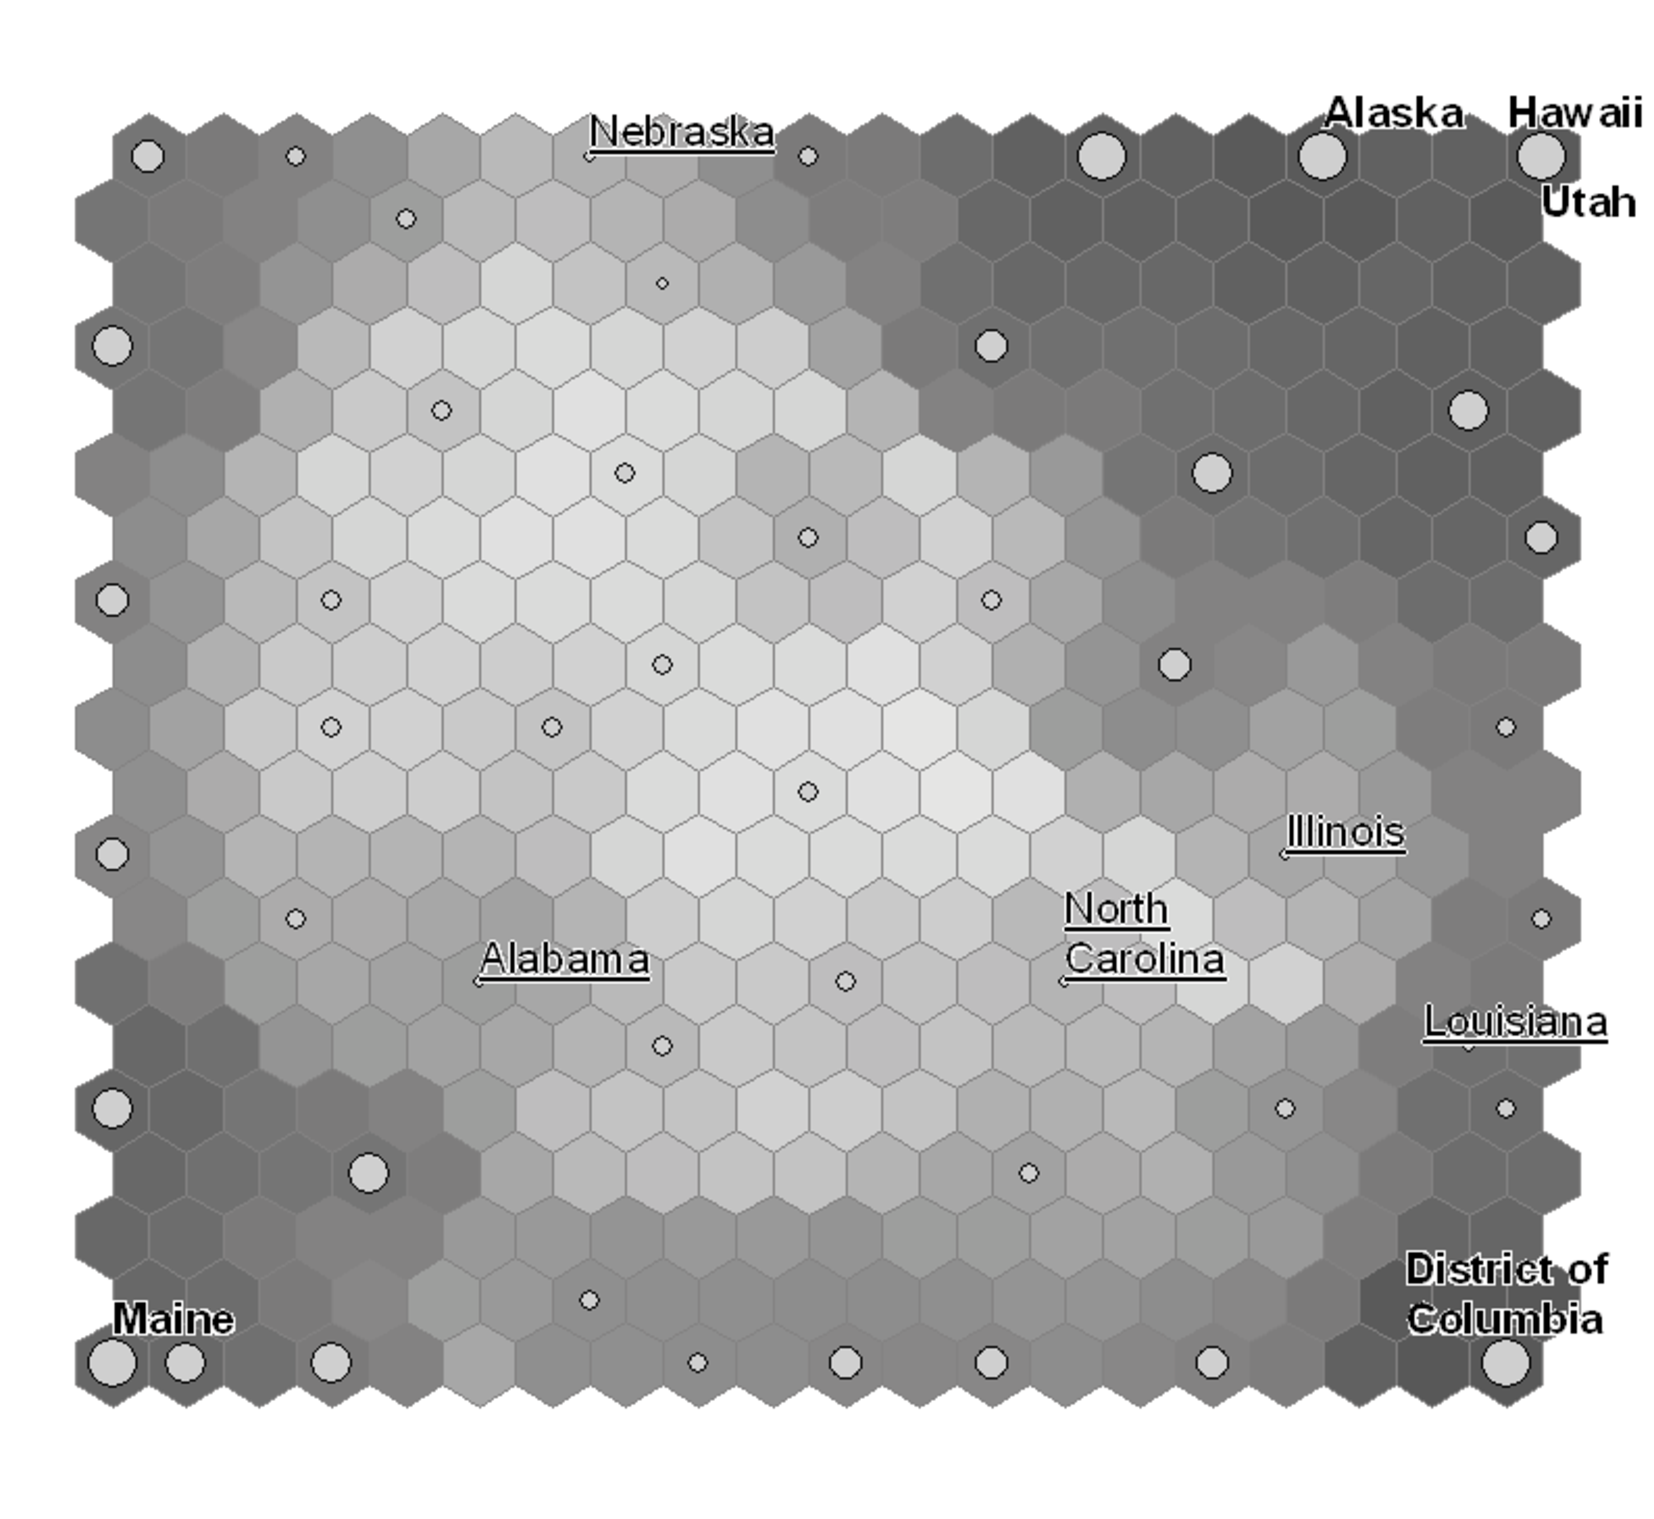
\includegraphics[width=\linewidth]{gridedge_grey.pdf}
\caption{Fifty States and the District of Columbia mapped onto a
SOM trained with thirty-two population census variables.  Darker neurons have a
relatively larger difference from the mean of the states, while lighter
neurons are relatively closer.  Smaller point symbols show states that are closer to the
mean, while large symbols show outliers. The five states closest to the average are shown
with underlined labels and the five states furthest from the mean are shown with
bold labels.}
\label{figure1}
\end{figure}

\section{Spherical SOM}
One way to eliminate the boundary effect is to wrap the lattice around a
three-dimensional object such as a sphere or torus, thereby removing the edge
entirely. The toroidal SOM was introduced by \cite{li1993}, however the torus is
not effective for visualization, as maps generated from a torus are not
very intuitive \citep{ito2000,wu2006}.  \cite{ritter99} describes the torus as
being topologically flat and suggests that a curved topology, such as that of a
sphere, may better reflect directional data.  A sphere also results in a more
intuitive map, since we are accustomed to looking at geographic maps based on a sphere.

\cite{ritter99} first introduced the spherical SOM, and several enhancements have
since been suggested \citep{boudjemai2003,sangole03,Nishio:2006fk,wu2006}.  A
good comparison of these enhancements can be found in \cite{wu2006}.  All of
these methods derive their spherical structure through the tessellation of a
polyhedron as originally proposed by \cite{ritter99}.  \cite{wu2006} point
out the importance of a uniform distribution on the sphere, and that it is
preferable for all neurons to have an equal number of neighbors and to be
equally spaced.  They find generally that the tessellation method best satisfies
these conditions, and specifically that the icosahedron is the best starting
point \citep{wu2005}. Tessellation of the icosahedron results in a network of
neurons, each of which having exactly six neighbors, save the original twelve
which each have five neighbors.  This is very close to the ideal structure in which every
neuron would have exactly six neighbors.  This structure has very low variances
in both neuron spacing and neighborhood size.

\section{Network Size}
\begin{figure}[htb]
\centering
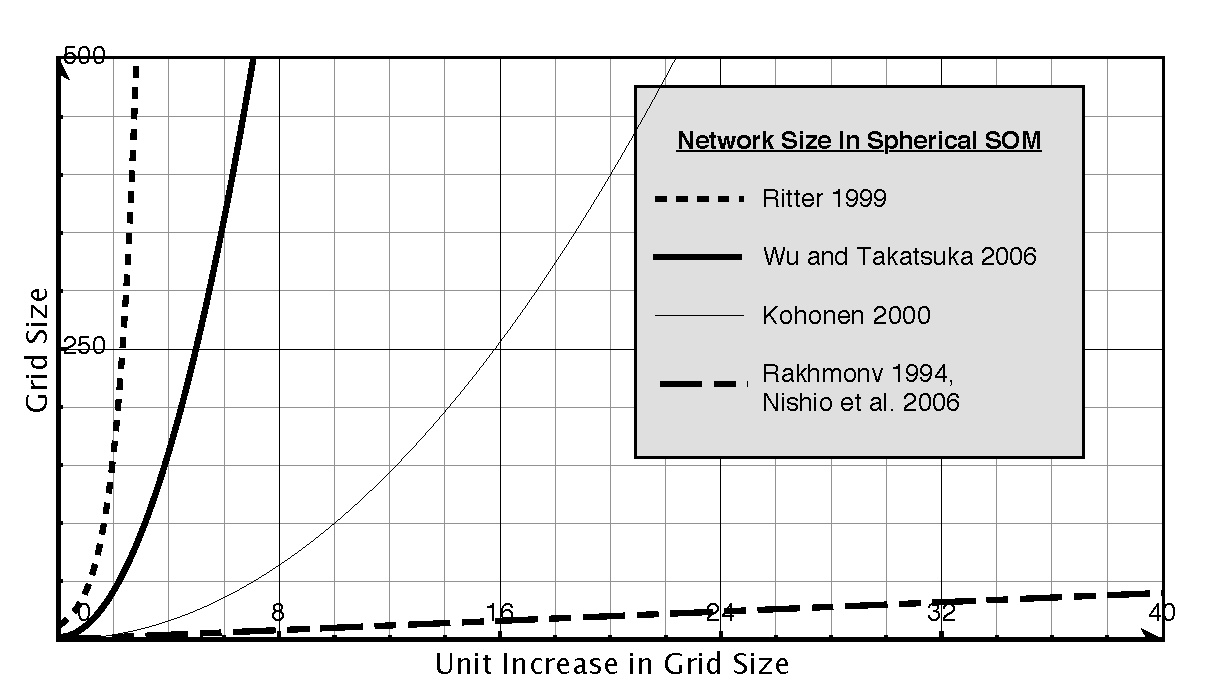
\includegraphics[width=\linewidth]{networkSize.pdf}
\caption{This figure demonstrates the achievable network size using various
spherical topologies, in comparison with the traditional SOM. The Y-axis represents the achievable network size, the
meaning of the X-axis is dependent on the topology. For the tessellation
methods the X-axis represents the frequency of the tessellation. For the
traditional Kohonen method the X-axis represents the size of both dimensions of
the grid; for comparability the ratio between the dimensions was fixed at one
($X_{dim}=Y_{dim}$).  For the \cite{Rakhmanov94} and \cite{Nishio:2006fk} methods the X-axis
represents the exact network size.}
\label{fig:nSize}
\end{figure}
The literature offers little theoretical guidance on choosing an appropriate
network size for a given dataset \citep{cho1996}.  \cite{toolbox} suggests
that the network size should be ``as big as possible,'' but also states that
this becomes computational impractical for larger problems. As a general
rule-of-thumb, the author suggests using a network size of \(5\sqrt {n}\),
where \(n\) is the number of observations. Given this lack of theoretical
development, researchers should be cautious when using methods that limit the
control of network size.  Having a high level of control over network size
allows support for such very different SOM applications as clustering versus
low-dimensional spatial layout.  \cite{skupin08} demonstrate this when they
use the same data to train two SOMs of different sizes.  In the three-by-three
(9) case the neurons act as containers clustering similar states, while in the
twenty-by-twenty (400) case relationships are expressed with much finer
granularity.  As shown in Figure \ref{fig:nSize}, the achievable network size
varies between topologies.

In rectangular and hexagon SOMs it is undesirable to have one
dimension drastically larger than another, as such there are practical
limitations to the size of these networks.  As an aside, the preferred ratio
between these dimensions depends on the data being represented, and should
generally not equal one \citep{kohonen1996, toolbox}. We use a ratio of one
only for comparison purposes with the other topologies.
\citeauthor{ritter99}'s tessellation method results in a network size that
grows at a rate of \(N=2+10*4^f\), where $f$ is the frequency of tessellation.
\cite{wu2006} offer a slight improvement. Rather than recursively subdividing
the faces, they redivide the original icosahedron with each step, resulting in
\(N=2+10*f^2\).  Methods for arranging an arbitrary number of points on a
sphere provide a much higher degree of flexibility when choosing a network
size.


This first five possible sizes of the geodesic SOM are; 12, 42, 92, 162 and 252.  

The cost of relying on \citeauthor{ritter99}'s tessellation method is
decreased control over network size. 

%In practice, 2D Euclidean SOMs also offer limited control over network size because it is undesirable to have one dimension dramatically larger than the other. 



\cite{Nishio:2006fk} try to address the
issue of network size granularity by departing from the tessellation method and
suggesting the use of a partitioned helix to uniformly distribute any number of
neurons on a sphere.  A similar method proposed by \cite{Rakhmanov94} was
dismissed by \cite{wu2005} for failing to satisfy the uniformity conditions
described above.


\section{Uniformity}
\citeauthor{wu2006} state that ``[f]or SOM, it is desirable to have all neurons
receive equal geometrical treatment'' \cite[p. 900]{wu2006}.  To satisfy this
constraint, two conditions must be met.  First, each neuron should occupy the
same amount of space on the given surface.  Second, each neuron should be
bordered by the same number of surrounding neurons, and we should maximize that
number.  The first condition may be important for visualization, but is
irrelevant for training.  During the training of the SOM only the topology of
the neurons is considered.

Based solely on measures of neuron spacing, \cite{wu2005} dismissed a method
proposed by \cite{Rakhmanov94} for distributing points on a sphere.  Similarly
\cite{Nishio:2006fk} use these variance measures to support their helix
algorithm for distributing points on a sphere.  Table \ref{table1} shows that
these metrics can be misleading and comparison across topologies may not be
consistent.
The traditional rectangular and hexagonal topologies have no variance in neuron
spacing, and the generally preferred hexagonal structure displays greater
variance in neighborhood size than the rectangular structure.  The torus, by
comparison, would have variance in neuron spacing, yet no variance in
neighborhood size.  The distance between two neurons is only considered during
the formation of the neural network.  At this stage the spacing is significant
as it plays a part in determining neuron adjacency. However, using this measure
to evaluate potential topologies for use in SOM may be misleading.

\begin{table}[htbp]
\caption{Variances in Topologies}
\begin{center}
\begin{tabular}{|c|c|c|c|}
\hline
Topology&Grid Size&Neuron Spacing&Variance in Neighborhood Size\\
\hline
Rectangular&9x18&1&0.2716\\
Hexagonal&9x18&1&1.2138\\
Tessellation&162&0.25319 - 0.31287& 0.0686\\
Rakhmanov&162&0.15779 - 0.30069& 0.2908\\
\hline
\end{tabular}
\end{center}
\label{table1}
\end{table}

Methods for distributing points on the sphere, which allow for fine-grained
control over network size, produce slightly more irregular topologies.  However,
no substantive discussion of these irregularities or their effects on SOM
training exists in the literature. Given that limited theoretical guidance is available
for choosing network size, the desire for finer control over the network size
should not be overlooked. Particularly for larger SOMs, the desired network size
may not be achievable via tessellation of the icosahedron.

